\subsection{Sensitive analysis of SI methods for the ship data}
\label{se:accuracy_SI_method}
Prior to the validation the behaviour of the SI-method was studied by varying the input parameters between minimum and maximum values in database around a point "reference ship" with values in the middle of the input boundaries (Eq. \ref{eq:SI_limits}) (see figure \ref{fig:SI_sensitivity}). It can be seen that the wave damping $B_W$ increases a lot with the absolute value of $OG/T$. It can also be seen the the wave damping has an enormous increase when the beam to draught ratio exceeds the input boundary, which seems to be the case for at least one third of the roll decay tests. It can also be noted that most of the ships in the database have midsection coefficients $A_0$ and bilge keel heights outside the limits. 

\begin{figure}[H]
    \centering
    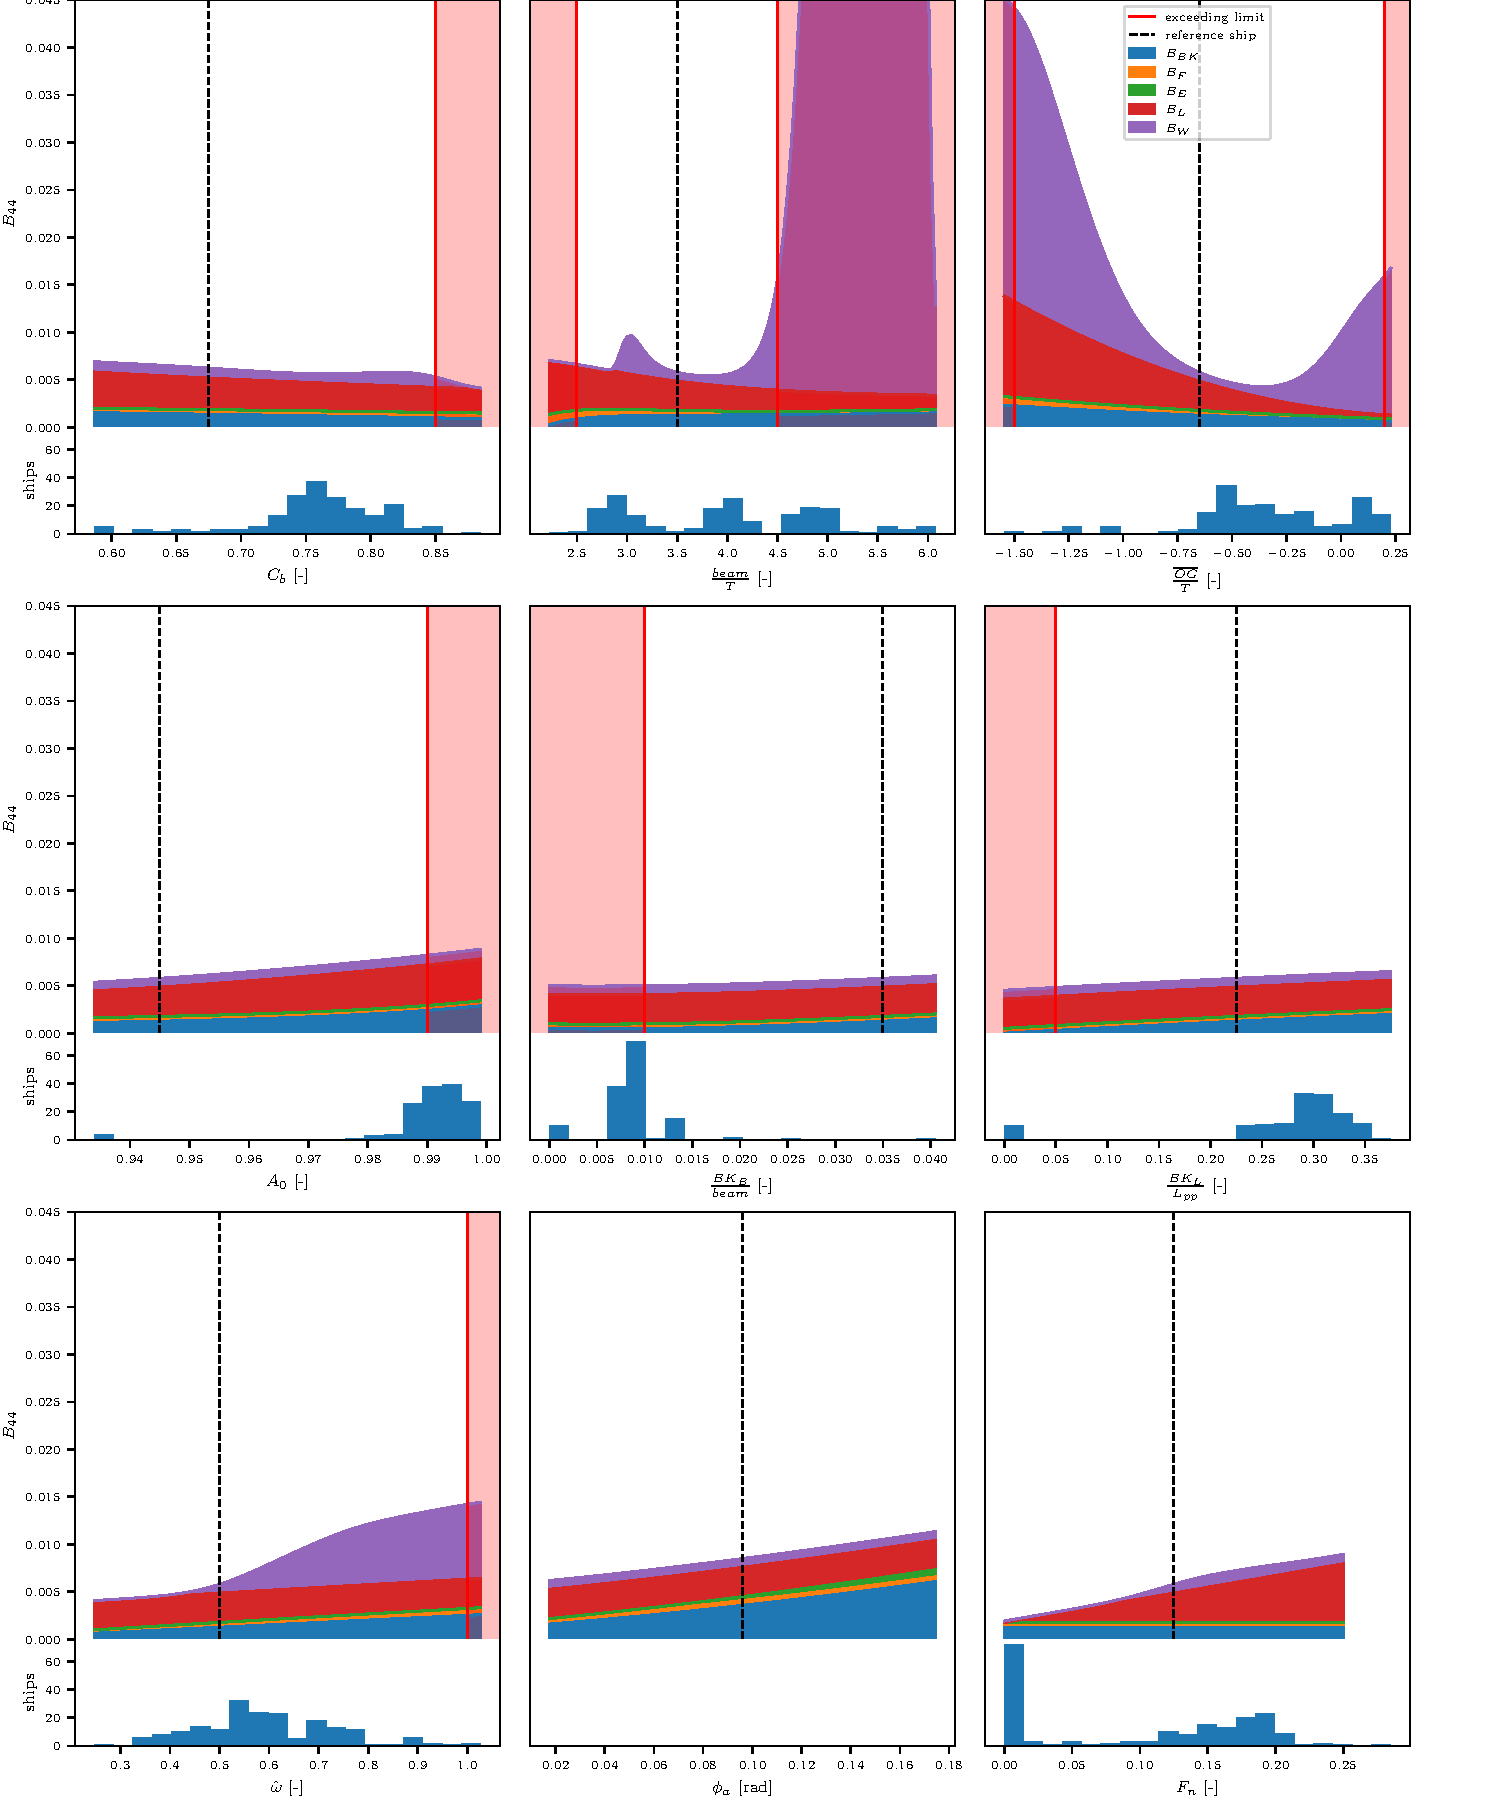
\includegraphics[width=\textwidth]{figures/SI-sensitivity.pdf}
        \vspace{-0.5cm}
    \caption{SI-method input parameter variation and data base ships}
    \label{fig:SI_sensitivity}
\end{figure}
